\documentclass[main]{subfiles}

\begin{document}

\section{Additional Topics}
This chapter discusses those topics that didn't fit in nicely anywhere in the script. If you, as a reader, find that these topics do fit in nicely elsewhere, possibly with some slight rearrangement of the topics, feel free to send us an email.
\subsection{Sorting Networks}
In this chapter we turn our attention to parallel sorting algorithms, which we'll represent using so-called \textit{sorting networks}. We'll see what common sorting algorithms look like when parallelized and how to prove or disprove that a sorting network actually sorts any arbitrary sequence of numbers correctly.\\[3mm]
We know that a sorting algorithm, with the exception of some specialized cases, cannot do better than $O(nlogn)$ in the worst case. The obvious next step is to try and break this lower bound by using the multiprocessors available to us, i.e. by parallelizing sorting algorithms.\\[3mm]
\begin{wrapfigure}{r}{.35\textwidth}
    \centering
    \vspace{-15pt}
    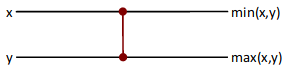
\includegraphics[scale=0.5]{Comparator.png}
\end{wrapfigure}
First off, we need to define what a sorting network looks like. To that end, we define the \textit{comparator}, which swaps two values, such that the higher value ends up at the bottom.\\[3mm]
We will now look at what good old Bubble Sort looks like as a sorting network. The idea of Bubble Sort is essentially that we first find the highest value among the first $n$ values of the array, then among the first $n-1$ values, and so on until we've sorted the entire array. As a sorting network, that looks like this:
\begin{figure}[H]
    \centering
    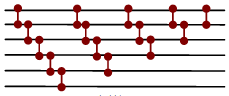
\includegraphics[scale=0.5]{BubbleSort.png}
\end{figure}Let’s take a quick break and think about what an actual actor could look like.
\noindent From this visual representation it's pretty obvious which comparators can be executed in parallel. We ''shift'' all the comparators as far to the left as possible without having several comparators act on the same variables simultaneously, as this would result in a data race. This gives us the following sorting network for parallel Bubble Sort:
\begin{figure}[H]
    \centering
    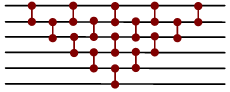
\includegraphics[scale=0.5]{ParallelBubbleSort.png}
\end{figure}Let’s take a quick break and think about what an actual actor could look like.
Given an infinite number of processors, parallel Bubble Sort will therefore take $2n-3$. We can improve this even further to $n$ by rearranging the comparators such that all ''even'' resp. all ''odd'' comparators operate in parallel. The algorithm can be improved even further, but that's far beyond the scope of this course.\\[3mm]
Having seen what a sorting network is we're now interested in proving that a particular sorting network will sort any arbitrary sequence of numbers. As there are of course infinitely many such sequences, we need some easier way of proving such a property. This leads us to the \textit{zero-one principle}.
\begin{theorem}
    If a network with $n$ input lines sorts all possible input sequences of 0s and 1s into a non-decreasing order, it will sort any arbitrary sequence of $n$ numbers in non-decreasing order.
\end{theorem}
By using this principle, we can prove the correctness of a given sorting network with relative ease.
\newpage
\begin{example}
    We're given the following sorting network:
\begin{figure}[H]
    \centering
    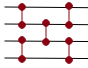
\includegraphics[scale=0.6]{SortingNetwork1.png}
\end{figure}
\noindent Tasked with determining whether this sorting network is correct or not, we turn our attention to the \textit{zero-one-principle}. 
For the sake of brevity, we'll skip ahead to the conclusion and see that it's actually not correct, as can be seen by the following sequence:
\begin{figure}[H]
    \centering
    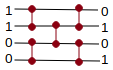
\includegraphics[scale=0.6]{SortingNetwork2.png}
\end{figure}
\end{example}

\newpage

\subsection{Transactional Memory}
We've learned how to correctly implement concurrent programs using locks, but a few problems still remain:
\begin{itemize}
    \item \textbf{Deadlocks}: Threads might attempt to acquire locks in a different order, thereby introducing a cyclic dependency
    \item \textbf{Convoying}: A thread might be descheduled while other threads queue up waiting for it to continue
    \item \textbf{Priority Inversion}: Lower priority threads might hold a resource that a higher priority thread is waiting for
    \item Association of data and locks is established by \textbf{convention}, i.e. a correct use of the program by future developers depends on reasonable documentation
    \item \textbf{Non-composable}: Changing anything about the locking scheme requires changing the whole program
    \item \textbf{Pessimistic by design}: Assumes the worst and introduces expensive mutual exclusion as a consequence
\end{itemize}
We might attempt to resolve some of these problems using compare-and-swap, but, as one might see when attempting to implement a lock-free sorted linked list, this is often not enough. Double-compare-and-swap could be enough, but at this point it's only a theoretical concept. We therefore need some way of allowing the programmer to declare a block of code atomic without placing a large burden on him.\\[3mm]
This is where \textit{transactional memory} comes into play. In transactional memory, we define atomic code sections called \textit{transactions}, which guarantee:
\begin{enumerate}
    \item \textbf{Atomicity}: Changes made by transactions are made visible atomically, i.e. other threads either observe the initial or final state, but nothing in between. Note that this is done without mutual exclusion.
    \item \textbf{Isolation}: While a transaction is running, effects from other transactions aren't observed.
\end{enumerate}
It is convenient to say something about how transactions are implemented. Transactions are executed \textit{speculatively}: as a transaction executes, it makes \textit{tentative} changes to objects. If it completes without a synchronization conflict, it \textit{commits} (the tentative changes become permanent) or it \textit{aborts} (the tentative changes are discarded.
\begin{example}
    As one might have seen during the lecture, implementing a concurrent bounded producer/consumer queue requires a lot of thought (see: Sleeping Barber). However, using transactions implementing one becomes nearly trivial. Below we've depicted the enqueue method of such a bounded queue.
    \begin{figure}[H]
        \centering
        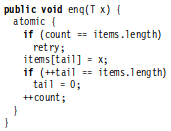
\includegraphics[scale=0.7]{Transaction_Ex.png}
    \end{figure}
    The method enters the \texttt{atomic} block, and tests whether the buffer is full or not. If so, it calls \texttt{retry}, which \textit{rolls back} the enclosing transaction, pauses it, and restarts it when the object's state has changed. If not, it enqueues the item, increments the index modular the length of the queue, and exits the \texttt{atomic} block.
\end{example}
Transactional memory sound fantastic, but where is it implemented? There have been attempts to implement transactional memory in hardware and while these implementations can certainly be fast, their resources are bounded and they can therefore often not handle larger transactions. The implementation that we will work with is directly in software in parallel programming languages, which allows for greater flexibility, though achieving good performance might be more challenging.

\subsubsection{Concurrency Control}
In order to guarantee that a running transaction always sees consistent data, transactional memory implements a \textit{concurrency control} (CC) mechanism. The CC will \textit{abort} a transaction when a \textit{conflict} occurs. An example of a conflict is a when a transaction that hasn't yet committed has read a value that is later changed by a committed transaction. Once a transaction is aborted, it can either be retried automatically (not necessarily immediately) or the user is notified. \\[3mm]
Synchronization conflicts cause transactions to abort, but it's not always possible to halt a transaction's thread immediately after the conflict occurs. Instead, such \textit{zombie} transactions may continue to run even after it has become impossible for them to commit. This raises the question: How do we prevent such a zombie from seeing an inconsistent state?
\begin{example}
    Such an inconsistent state could arise if an object has two fields $x$ and $y$, where each transaction preserves the invariant that $x > y$. Transaction \textbf{Z} reads $y$, and sees the value 2. Transaction \textbf{A} changes $x$ and $y$ to 1 and 0, respectively, and commits. Suppose \textbf{Z} keeps running, i.e. \textbf{Z} is a zombie, since it will never commit. \textbf{Z} will later see an inconsistent state, when it reads the value 1 for $x$.\\[3mm]
    One might be tempted to say we can ignore this problem, as \textbf{Z} will never commit anyways, i.e. its updates will be discarded. But unfortunately, life isn't that easy. Let's say that after reading $x$, \textbf{Z} computes the value for $\sqrt{x-y}$. Under normal circumstances, evaluating this expression shouldn't throw an exception. \textbf{Z} has read an inconsistent state and will now throw an exception, which, depending on the implementation, could crash the program.
\end{example}
As there is no ''practical'' way of preventing exceptions in a programming model where invariants such as $x > y$ cannot be relied on, Transactional memory systems mostly guarantee that all transactions, even zombies, see consistent states.\\[3mm]
Transactional memory organizes mutable state into \textit{atomic objects}, to which it associates \textit{timestamps}, which indicates when the object was last changed by a committed transaction. A transaction will keep a local \textit{read-set} and a local \textit{write-set}, holding all locally read and written objects, respectively. When a transaction calls \textit{read}, it will check if the object is in the write-set and use this new version if it is. If not, it will check if the object's time stamp is smaller than the transaction's birthdate. If the object has been changed by some other transaction after the transaction's birthdate, it will abort. Otherwise, it'll add a new copy of the object to the read-set. When a transaction calls \textit{write}, it'll create a copy of the object in the write-set, if there isn't one already.\\[3mm]
When a transaction attempts to commit, all objects of the read-set and write-set are locked, and the timestamps of the objects in the read-set are compared to the birthdate of the transaction. If any of the objects were changed after the transaction started, it's aborted. Otherwise, all objects in the write-set are copied back to global memory with their new timestamps. All locks are released and a ''commit'' is returned.

\subsubsection{Scala-STM}
\textit{ScalaSTM} is a Java API through which we can access the methods provided by the Scala STM library. ScalaSTM is a so-called \textit{reference-based STM}, which means that mutable state, i.e. state which can only be modified \textit{inside a transaction}, is put into special variables.
\begin{center}
    \texttt{private final Ref.View$<$Integer$>$ count = STM.newRef(0);}
\end{center}
Arrays can be declared as follows:
\begin{center}
    \texttt{private TArray.View$<$E$>$ items = STM.newTArray(capacity);}
\end{center}
Everything else is immutable, which means any other variable accessed inside an atomic block must be declared \texttt{final}.\\[3mm]
We can create an atomic block as follows:
\begin{center}
    \texttt{STM.atomic(new Runnable()\{...\});}\quad or\quad \texttt{STM.atomic(new Callable$<$T$>$()\{...\});}
\end{center}
Note that the passed \texttt{Runnable} or \texttt{Callable} object must implement the \texttt{public void run()} or the \texttt{public T call()} method, respectively.\\[3mm]
\begin{example}
    We can now try to implement the \texttt{enq()} method of the bounded queue using ScalaSTM.\\[3mm]
    First, we need to distinguish between mutable state and immutable state. We see that we modify the variables \texttt{count, tail} and \texttt{items}. As these variables should indeed only be accessed from within a transaction, they are part of the mutable state. The method also accepts a parameter \texttt{x}. As we only read object and don't actually try to modify, we'll include it in the immutable state. All in all, our class will look something like this (omitting the other methods for brevity): 
    \begin{figure}[H]
        \centering
        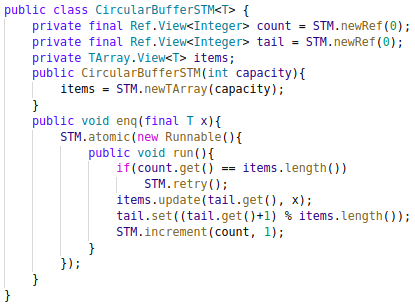
\includegraphics[scale=0.45]{CircularBufferSTM.png}
    \end{figure}
    
\end{example}

\newpage

\subsection{Message Passing}
We've now seen a lot of different ways of dealing with processes concurrently accessing the same data and we've come to one definite conclusion, it's hard. We might try to avoid sharing state by partitioning the dataset using the \texttt{ForkJoin} framework, we might use locks to guarantee consistency or we might even work with transactional memory, but all of these approaches are still difficult to work with, near impossible to implement or both. Taking a step back, we see that the root cause of the problem is the fact that we have shared mutable state. So, what if we didn't? This is the core idea of \textit{message passing}, namely to have processes run in isolation and only communicate via messages which must be explicitly received.

\subsubsection{Message Passing Interface}
The \textit{Actor Model} is a model for concurrent computation. It uses \textit{actors} as computational agents which react to received messages. Received messages are mapped to a set of messages sent to other actors, a new behavior and a set of new actors created. In other words (and slightly informal), an actor is a thread which reacts to received messages and has a local state.
\begin{example}
    Let's take a quick break and think about what an actual actor could look like.\\[3mm]
    A \textbf{distributor} is a type of actor which forwards received messages to a set of actors in a round-robin fashion. There are two questions that we need to answer to be able to model an actor. What \textit{local state} should be kept by the actor and what should the actor do upon receiving a message? \\[3mm]
    The first question can be answered quickly. We know that we have a set of actors. In order to guarantee that the messages are distributed in a round-robin fashion, we store the actors in an array and we keep an index which indicates the entry in the array which contains the next actor to send a message to.\\[3mm]
    Now that we know what internal state we're going to keep, defining the behavior of the actor upon receiving a message seems obvious. The message can immediately be forwarded to the actor stored in the array entry indicated by the stored index. Then, we increment the index modular the array length. We also need to consider adding control commands which could, for example, allow us to add or remove actors from the set of stored actors.
\end{example}
Note that in the actor model messages are sent in an \textit{asynchronous fashion}, i.e. the sender places the message into the buffer of the receiver and continues execution. In contrast, when the sender sends \textit{synchronous} messages, it blocks until the message has been received.\\[3mm]
As always, Java has a library for it. The \textit{Message Passing Interface} (MPI) is a library which provides us with a message passing API which we can use to write message-passing programs.\\[3mm]
MPI collects processes into groups, where each group can have multiple ''colors'' and a group paired with its color uniquely identifies a communicator. Initially, all processes are collected in the same group and communicator \texttt{MPI\_COMM\_WORLD}. Within each communicator, a process is assigned a unique number to identify it by, called a \textit{rank}.
\subsubsection{Point-to-Point Communication}
The methods to send and receive messages are declared as follows:
\begin{figure}[H]
    \centering
    \begin{subfigure}{.5\textwidth}
        \centering
        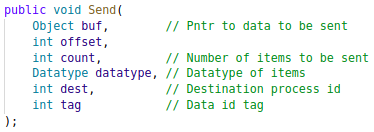
\includegraphics[scale=0.45]{MPI_Send.png}
    \end{subfigure}%
    \begin{subfigure}{.5\textwidth}
        \centering
        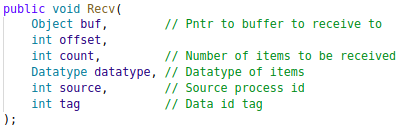
\includegraphics[scale=0.45]{MPI_Recv.png}
    \end{subfigure}
\end{figure}
Note that in the case of the \texttt{Recv} method it's not necessary to declare \texttt{src} or \texttt{tag}, instead one could use \texttt{MPI\_ANY\_SOURCE} or \texttt{MPI\_ANY\_TAG}. Both methods are declared in the \texttt{COMM} class, i.e. can only be used in combination with a communicator.\\[3mm]
The two methods declared above are so-called \textit{blocking} operations, which means they won't return until the action has been completed \textit{locally}. Their \textit{non-blocking} variants \texttt{recv} and \texttt{send} return \textit{immediately}. We can also send synchronous messages, i.e. the operation blocks until the message has been received, using \texttt{Ssend}. Note that the \texttt{Recv} method declared above already is synchronous.\\[3mm]
To summarize and complete what we've learned up until now, we can write a simple MPI program using the following six functions:
\begin{itemize}
    \item \texttt{MPI.Init()}: initialize the MPI library (first routine called)
    \item \texttt{MPI.COMM.Size()}: get the size of a communicator \texttt{COMM}
    \item \texttt{MPI.COMM.Rank()}: get the rank of the calling process in the communicator
    \item \texttt{MPI.COMM.Send()}: Send a message to another process in the communicator
    \item \texttt{MPI.COMM.Recv()}: Receive a message from another process in the communicator
    \item \texttt{MPI.Finalize()}: Clean up all MPI state (last routine called)
\end{itemize}
\begin{example}
    Given an array of integers, let's compute the number of prime factors for each entry. The resulting array should be present in the process with rank 0 at the end. For simplicity, assume the array length is divisible by the number of processes.
    \begin{figure}[H]
        \centering
        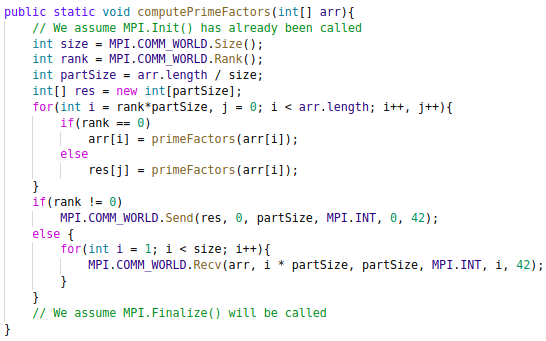
\includegraphics[scale=0.45]{MPI_Ex.png}
    \end{figure}
\end{example}
\subsubsection{Group Communication}
Up until now we've only considered communication between two specific processes. MPI also supports communications among groups of processes. In theory, this isn't really necessary to write a program, but it is essential to performance.\\[3mm]
\texttt{MPI.COMM.Reduce()} takes an array of input elements on each process and returns an array of output elements to the specified root process. The output elements contain the reduced result. \texttt{MPI.COMM.ReduceAll()} does the exact same thing, only returning the result to all processes instead of a single root process.\\[3mm]
\begin{figure}[H]
    \centering
    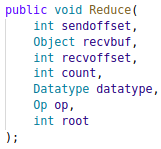
\includegraphics[scale=0.45]{MPI_Reduce.png}
\end{figure}
\texttt{MPI.COMM.Scan()} takes an array of input elements on each process and returns distinct arrays of output elements to each process, where the operation is applied iteratively, with the final result array being returned to the specified root process. The method declaration is identical to the declaration of \texttt{Reduce()}, but for the method name.\\[3mm]
Using \texttt{MPI.COMM.Bcast()} one process can \textit{broadcast}, i.e. send, the same data to all processes in a communicator. Note that both the receiver and sender processes call the same method.
\begin{figure}[H]
    \centering
    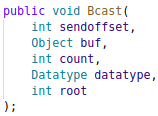
\includegraphics[scale=0.45]{MPI_Bcast.png}
\end{figure}
Finally, we arrive at the \texttt{MPI.COMM.Scatter()} and \texttt{MPI.COMM.Gather()} methods. \texttt{Scatter()} involves a root process sending data to all processes in a communicator. The main difference to \texttt{Bcast()} is that \texttt{Scatter()} sends \textit{chunks of an array} to different processes, while \texttt{Bcast()} sends the \textit{entire array} to all processes. \texttt{Gather()} does the exact inverse of \texttt{Scatter()}, in that it takes data from many processes and gathers them to a single root process. The elements are ordered by the rank of the process from which they were received.
\begin{figure}[H]
    \centering
    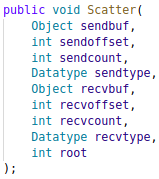
\includegraphics[scale=0.45]{MPI_Scatter.png}
\end{figure}

It's important to know that the method declarations aren't necessarily accurate, as there are many different MPI implementations with variations in parameters and parameter ordering.

\newpage

\subsection{Exercises}
% Add exercise about transaction zombies
\begin{ExerciseList}
    \Exercise[title={Sorting Networks},label=SN].\quad \\
        \Question How many inputs does one have to check correctness of a sorting network that takes integer inputs of length 4, using the 0-1 principle?
        \Question For each of the following sorting networks, decide whether they're correct. If not, give a counterexample.
            \begin{figure}[H]
                \centering
                \begin{subfigure}{.5\textwidth}
                    \centering
                    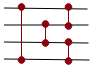
\includegraphics[scale=0.7]{SN1.png}
                    \caption{}
                \end{subfigure}%
                \begin{subfigure}{.5\textwidth}
                    \centering
                    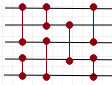
\includegraphics[scale=0.7]{SN2.png}
                    \caption{}
                \end{subfigure}
                \begin{subfigure}{.5\textwidth}
                    \centering
                    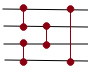
\includegraphics[scale=0.7]{SN3.png}
                    \caption{}
                \end{subfigure}%
                \begin{subfigure}{.5\textwidth}
                    \centering
                    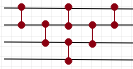
\includegraphics[scale=0.7]{SN4.png}
                    \caption{}
                \end{subfigure}
            \end{figure}
        \Question Draw the parallel sorting network corresponding to insertion sort for an input sequence of length 5.
    
    \Answer[ref={SN}].\quad \\
        \Question The 0-1 principle states that if the network sorts all possible input sequences of 0s and 1s into a non-decreasing order, it will sort any arbitrary sequence of input numbers in a non-decreasing order. As there are $2^n$ possible input sequences of length $n$ of 0s and 1s, one has to check 16 sequences to ensure correctness of the sorting network.
        \Question 
            \begin{enumerate}[label=(\roman*)]
                \item This sorting network is incorrect, as can be seen by the following incorrectly sorted input sequence.
                \item This sorting network is incorrect, as can be seen by the following incorrectly sorted input sequence.
                \item This sorting network is incorrect, as can be seen by the following incorrectly sorted input sequence.
                \begin{figure}[H]
                    \centering
                    \begin{subfigure}{.5\textwidth}
                        \centering
                        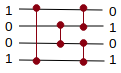
\includegraphics[scale=0.7]{SN1_sol.png}
                        \caption{}
                    \end{subfigure}%
                    \begin{subfigure}{.5\textwidth}
                        \centering
                        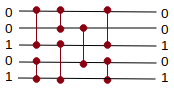
\includegraphics[scale=0.7]{SN2_sol.png}
                        \caption{}
                    \end{subfigure}
                    \begin{subfigure}{.5\textwidth}
                        \centering
                        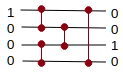
\includegraphics[scale=0.7]{SN3_sol.png}
                        \caption{}
                    \end{subfigure}
                \end{figure}
                \item We see that this sorting network is a parallelized version of bubble sort. Checking all 16 possible input sequences yields the expected result: the network is correct.
            \end{enumerate}
        \Question The sequential sorting network corresponding to insertion sort looks as depicted in (i). ''Shifting'' the comparators as far t0 the left as possible to obtain the maximum amount of parallelism gives us (ii). Interestingly  enough, this sorting netwrk is identical to the sorting network we obtain when parallelizing bubble sort.
            \begin{figure}[H]
                \centering
                \begin{subfigure}{.5\textwidth}
                    \centering
                    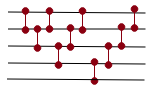
\includegraphics[scale=0.7]{InsertSort_Seq.png}
                    \caption{}
                \end{subfigure}%
                \begin{subfigure}{.5\textwidth}
                    \centering
                    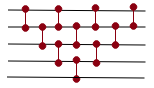
\includegraphics[scale=0.7]{InsertSort_par.png}
                    \caption{}
                \end{subfigure}
            \end{figure}
    
    
    \Exercise[title={Software Transactional Memory}, label=STM]. \quad \\
        \Question Implement the \texttt{deq} method of the \texttt{CircularBufferSTM$<$T$>$} class.
        \Question Implement a bounded stack (i.e. a stack which isn't allowed to grow past a certain size) using ScalaSTM.
        %\Question Implement a sorted linked list using ScalaSTM.
    
    \Answer[ref={STM}]. \quad \\
        \Question We add a \texttt{head} variable which tracks the front of the queue and use a \texttt{Callable} class instead of a \texttt{Runnable}, as we need to be able to return a result.
            \begin{figure}[H]
                \centering
                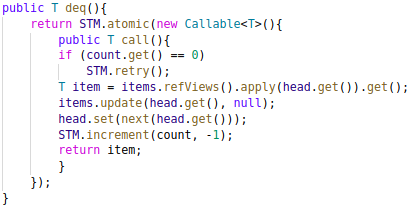
\includegraphics[scale=0.45]{CircularBufferSTM_deq.png}
            \end{figure}
        \Question Our implementation is nearly identical to the previously implemented \texttt{CircularBuffer}, only we don't need to track a tail and head of the buffer, but only the number of items on the stacks. As we know the maximum size of the stack in advance, we store the items in an array.
            \begin{figure}[H]
                \centering
                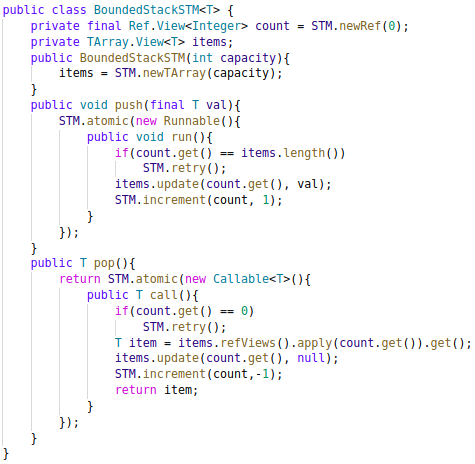
\includegraphics[scale=0.45]{BoundedStackSTM.png}
            \end{figure}

    
    \Exercise[title={Message Passing},label=MPI]. \quad \\
        \Question Adapt the \texttt{computePrimeFactors} method such that the resulting array is present in all processes at the end. \textit{Hint: Look up the \texttt{Allgather} method.}
        \Question Implement a method \texttt{randAvg} that works as follows:
            \begin{enumerate}
                \item Generate a random array of numbers on the root process (process 0).
                \item Distribute the numbers among all processes, giving each process an equal-sized chunk of the array. Assume that the array length is divisible by the number of processes.
                \item Each process computes the average of their subset of the numbers.
                \item Gather all averages to the root process. The root process then computes the average of these numbers to get the final average.
            \end{enumerate}
    
    \Answer[ref={MPI}]. \quad
        \Question We use the \texttt{Allgather} method to make the code more concise.
            \begin{figure}[H]
                \centering
                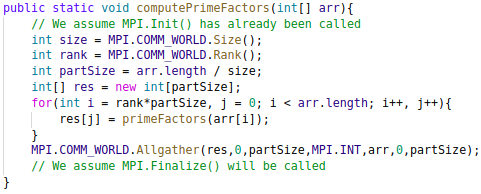
\includegraphics[scale=0.45]{computePrimeFactorsV2.png}
            \end{figure}
            Given a set of elements distributed across all processes, \texttt{Allgather} will gather all of the elements to all the processes. In the most basic sense, \texttt{Allgather} is a \texttt{Gather} followed by a \texttt{Bcast}.
        \pagebreak
        \Question We use the \texttt{scatter} and \texttt{gather} methods to compute the final average efficiently.
        \begin{figure}[H]
            \centering
            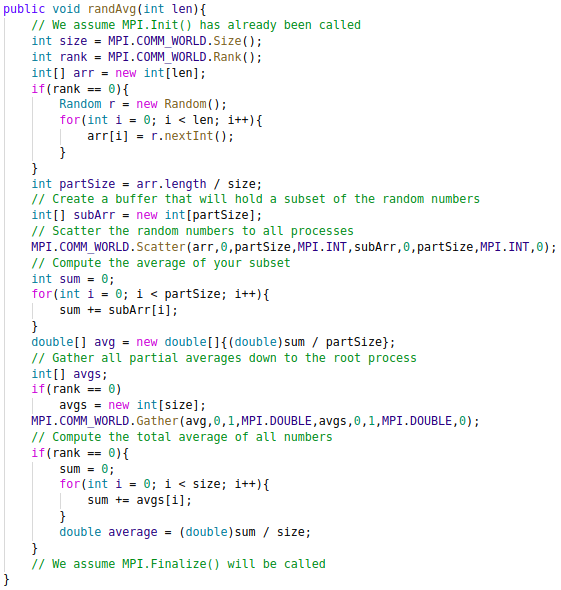
\includegraphics[scale=0.45]{randAvg.png}
        \end{figure}
\end{ExerciseList}
\newpage
\subsection{Solutions}
\shipoutAnswer
\end{document}